\documentclass[runningheads,a4paper]{llncs}

\usepackage[portuguese]{babel}
\usepackage[utf8]{inputenc}
\usepackage{amssymb}
\setcounter{tocdepth}{3}
\usepackage{graphicx}
\usepackage{url}
\usepackage{indentfirst}
\usepackage{float}

\begin{document}

\mainmatter  % start of an individual contribution

% first the title is needed
\title{Kropki}

% a short form should be given in case it is too long for the running head
\subtitle{Resolução de um problema de decisão usando Programação em Lógica com Restrições}
\titlerunning{Kropki}

% the name(s) of the author(s) follow(s) next
%
% NB: Chinese authors should write their first names(s) in front of
% their surnames. This ensures that the names appear correctly in
% the running heads and the author index.
%
\author{António Ramadas\and Rui Vilares}
%
\authorrunning{António Ramadas\and Rui Vilares}
% (feature abused for this document to repeat the title also on left hand pages)

% the affiliations are given next; don't give your e-mail address
% unless you accept that it will be published
\institute{Faculdade de Engenharia da Universidade do Porto\\
Rua Roberto Frias, sn, 4200-465 Porto, Portugal\\}

%
% NB: a more complex sample for affiliations and the mapping to the
% corresponding authors can be found in the file "llncs.dem"
% (search for the string "\mainmatter" where a contribution starts).
% "llncs.dem" accompanies the document class "llncs.cls".
%

\toctitle{Kropki}
\maketitle


\begin{abstract}

Este artigo complementa o segundo projeto da Unidade Curricular de Programação em Lógica, do Mestrado Integrado em Engenharia Informática e de Computação. O objetivo deste trabalho é construir um programa usando Programação em Lógica com Restrições para a resolução de um problema de decisão combinatória, o \textit{Kropki}. Conclui-se que, usando restrições, este jogo é relativamente fácil de reproduzir.

\keywords{kropki, sicstus, prolog, PLR, feup}

\end{abstract}


\section{Introdução}

O objetivo deste trabalho é a construção de um programa em Programação em Lógica com Restrições para a resolução de um dos problemas de otimização ou decisão combinatória sugeridos. O nosso grupo optou por um problema de decisão, o \textit{Kropki}.
 
O sistema de desenvolvimento é o SICStus Prolog, que inclui um módulo de resolução de restrições sobre domínios finitos: clp(FD).

Este artigo descreve detalhadamente a implementação do \textit{Kropki} em Prolog. São abordadas as variáveis de decisão e restrições utilizadas na resolução deste jogo. A estratégia de pesquisa e a visualização da solução são também tópicos importantes. Consideramos essencial acrescentar também estatísticas de resolução com diferentes complexidades. Finalmente, apresentamos os resultados obtidos, a conclusão e perspetivas de desenvolvimento.

\section{Descrição do Problema}

O Kropki é um quebra-cabeças baseado na colocação lógica de números. É utilizado um tabuleiro quadrado, de tamanho N. O objetivo do jogo é colocar números de 1 a N em cada uma das células vazias, de maneira que cada coluna e linha contenha os números de 1 a N apenas uma vez.

\begin{figure}[H]
	\centering
	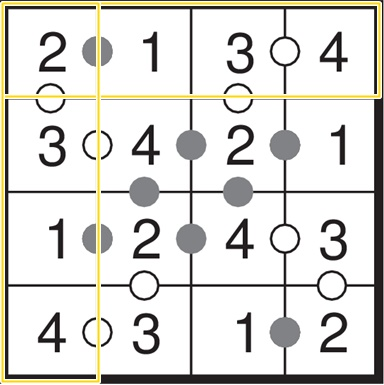
\includegraphics[scale=0.5]{images/rowCol.jpg}
	\caption{Exemplo da distribuição em linhas e colunas.}
	\label{fig:rowCol}
\end{figure}  
	
Além disso, se dois números consecutivos aparecerem em células vizinhas, são separados por um ponto branco. 

\begin{figure}[H]
	\centering
	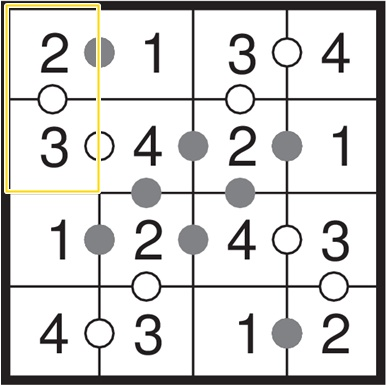
\includegraphics[scale=0.5]{images/whiteDot.jpg}
	\caption{Exemplo de um ponto branco.}
	\label{fig:whiteDot}
\end{figure}      

Se um número numa célula é metade do número da célula vizinha, então eles são separados por um ponto preto.

\begin{figure}[H]
	\centering
	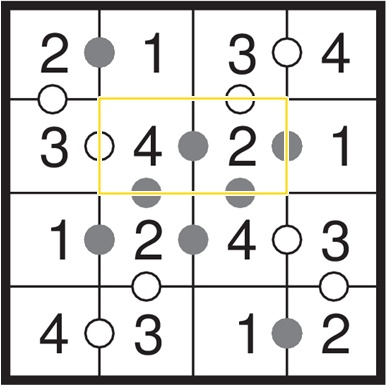
\includegraphics[scale=0.5]{images/blackDot.jpg}
	\caption{Exemplo de um ponto preto.}
	\label{fig:blackDot}
\end{figure}

\section{Abordagem}

A implementação do tabuleiro em Prolog foi baseada numa matriz. Assim, representamos o tabuleiro como uma lista de listas, onde cada elemento é número correspondente aquela célula.

\begin{figure}[H]
	\centering
	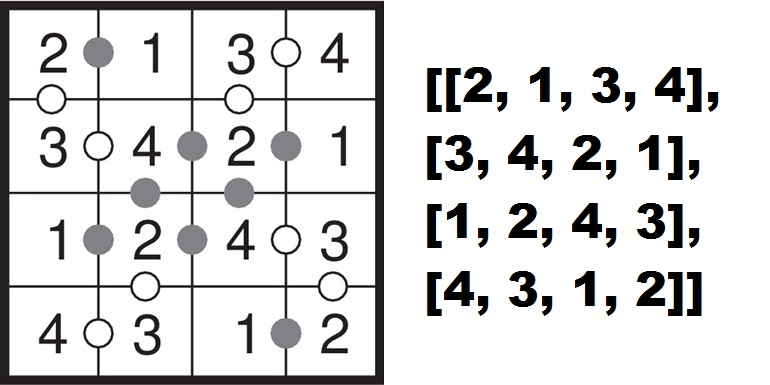
\includegraphics[scale=0.5]{images/representation.jpg}
	\caption{Representação interna.}
	\label{fig:representation}
\end{figure}

A representação interna dos pontos brancos e pretos faz-se recorrendo a \textit{asserts}.  

\begin{figure}[H]
	\centering
	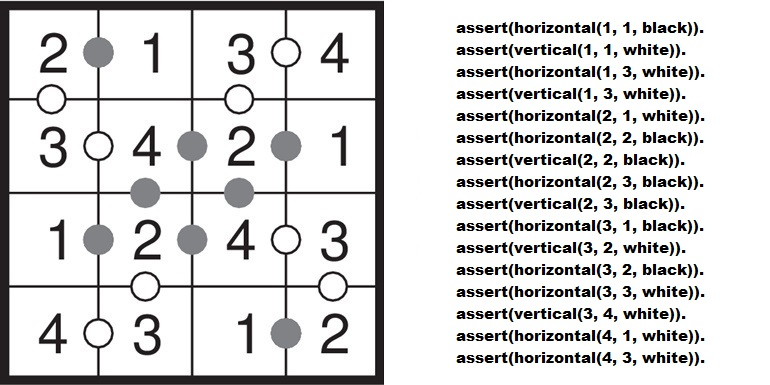
\includegraphics[scale=0.5]{images/asserts.jpg}
	\caption{Representação dos pontos.}
	\label{fig:dotRepresentation}
\end{figure}

\subsection{Variáveis de Decisão}

Com a representação utilizada, a solução apresenta-se sob a forma de uma lista de listas, todas elas com tamanho N. São também adicionados P pontos, representados através de clausulas, adicionadas pelo comando \textit{assert}.

Cada clausula guarda a informação de um determinado ponto, através da orientação referencial (vertical ou horizontal) em relação a uma célula específica (linha, coluna). Esse ponto encontra-se sempre entre a célula específica e a célula vizinha à sua direita ou a célula vizinha em baixo.

Sendo \textbf{N} o tamanho do tabuleiro e \textbf{P} o número de pontos distribuídos pelo tabuleiro, estas são as duas únicas variáveis que determinam o tamanho da solução.   

O domínio da solução é definido pela dimensão do tabuleiro. As linhas e as colunas variam de 1 a N e quantos mais pontos tiver o tabuleiro, mais complexa a solução se torna.

\subsection{Restrições}

A resolução do problema pode ser resumida às seguintes restrições:

\subsubsection{Cada linha deve conter os números de 1 a N apenas uma vez}\paragraph{}

Para um tabuleiro de tamanho N, percorrem-se recursivamente as linhas de 1 a N, e verifica-se se todos os números dessa linha são diferentes.

\subsubsection{Cada coluna deve conter os números de 1 a N apenas uma vez}\paragraph{}

Na verificação das colunas a situação é semelhante às linhas. Para um tabuleiro de tamanho N, calcula-se a matriz transposta e procede-se de forma análoga às linhas. 

\subsubsection{Com um ponto branco entre dois números, esses números têm que ser consecutivos}\paragraph{}

Quando estamos perante um pronto branco, é necessário verificar se o número \textbf{X} que preenche a célula especificada e o número que preenche a célula vizinha são consecutivos, ou seja, o número que preenche a célula vizinha terá que ser \textbf{X+1} ou \textbf{X-1}.   

\subsubsection{Com um ponto preto entre dois números, um números é metade do outro}\paragraph{}

Quando estamos perante um pronto preto, é necessário verificar se o número \textbf{X} que preenche a célula especificada é metade ou o dobro do número que preenche a célula vizinha, ou seja, o número que preenche a célula vizinha terá que ser \textbf{X/2} ou \textbf{X*2}.  

\paragraph{}
A implementação destas restrições em Prolog é assegurada pelos predicados apresentado de seguida. 

\begin{verbatim}
% Verifica se cada coluna e linha contêm os números de 1 a N apenas uma vez.
setDifferent(Board, SolvedBoard),

% Verifica as restrições impostas pelos pontos pretos e brancos.
setAsserts(SolvedBoard, 1, 1, Size)
\end{verbatim}

\subsection{Estratégia de Pesquisa}

Descrever a estratégia de etiquetagem utilizada é importante para perceber a eficiência do programa.

Na criação do tabuleiro de forma aleatória, é usado \textbf{labeling([variable(sel)], Board)}. O sel é um predicado, que escolhe um elemento de uma lista de forma aleatória.

Para resolver o tabuleiro utilizamos \textit{labeling} com opção ffc, que começa por atribuir valores às variáveis com o domínio mais pequeno.

\section{Visualização da Solução}

Os predicados responsáveis pela visualização dos possíveis tabuleiros do puzzle em modo texto, apesar de serem uma grande parte do código, foram relativamente fáceis de implementar. O facto de termos trabalhado com uma representação semelhante no passado, acabou por facilitar o desenvolvimento desta.

\begin{figure}[H]
	\centering
	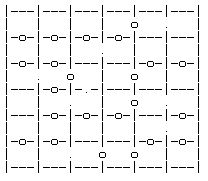
\includegraphics[scale=0.8]{images/unsolved.jpg}
	\caption{Representação de um tabuleiro, por resolver.}
	\label{fig:unsolved}
\end{figure}

\begin{figure}[H]
	\centering
	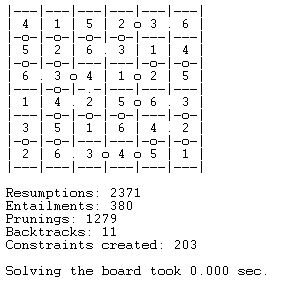
\includegraphics[scale=0.8]{images/solved.jpg}
	\caption{Representação de um tabuleiro, resolvido.}
	\label{fig:solved}
\end{figure}

Todo o código relativo à visualização do tabuleiro encontra-se no ficheiro \textit{display.pl}. O tabuleiro apresentado na consola é facilmente entendido, no entanto, é importante esclarecer que o símbolo "\textbf{o}" representa os pontos brancos e o símbolo "\textbf{.}" os pretos.       

O tabuleiro está a ser impresso linha a linha e para cada elemento é verificado o ponto à sua direita e em baixo. O predicado responsável por desenhar o tabuleiro é o \textbf{printBoard(Board)}. Os pontos que surgem na vertical de cada célula, são impressos pelo predicado \textbf{printDotVertical}, chamado em \textbf{printLine}. Os pontos que surgem na horizontal da célula, são impressos pelo predicado \textbf{printDotHorizontal}, chamado em \textbf{printLineNumbers}. Os elementos do tabuleiro, são impressos pelo predicado \textbf{printElem(Elem)}. 

Juntamente com o tabuleiro resolvido são apresentadas as estatísticas, através do predicado \textbf{fd\_statistics}. Isto permite uma melhor análise e discussão dos resultados.    

\section{Resultados}

Para testar a aplicação desenvolvida, corremos-la 5 vezes com cada tamanho N e apontamos o tempo que cada uma delas demora a encontrar a solução. Depois, usamos esses valores para calcular a média e elaborar um gráfico. 

\begin{figure}[H]
	\centering
	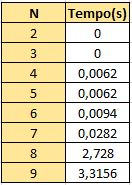
\includegraphics[scale=0.7]{images/table.jpg}
	\caption{Média dos tempos obtidos para cada tamanho do tabuleiro.}
	\label{fig:table}
\end{figure}

\begin{figure}[H]
	\centering
	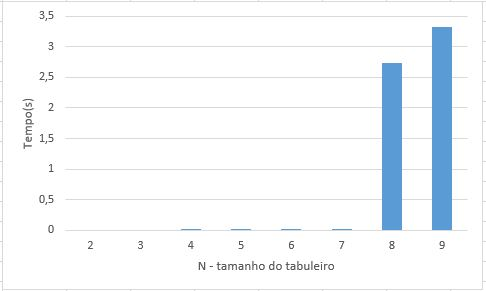
\includegraphics[scale=0.7]{images/graph.jpg}
	\caption{Gráfico com os dados obtidos.}
	\label{fig:graph}
\end{figure}
 
Os resultados obtidos nos testes foram encarados com naturalidade, uma vez que já eram espetáveis. Com o aumento do tamanho do tabuleiro, o tempo de resolução aumenta drasticamente. Os testes com o tamanho do tabuleiro superior a 10 tornam-se inviáveis, já que demoram muito tempo a ser resolvidos, dada a sua complexidade. 

\section{Conclusões e Trabalho Futuro}

O resultado final aqui apresentado orgulha-nos imenso. Para além de reproduzirmos, com qualidade, o \textit{Kropki}, satisfazemos todas as condições associadas a este jogo com uma eficiência, a nível de resolução, muito considerável.

O uso de PLR (Programação em Lógica com Restições) é muito útil para determinadas situações, uma vez que, facilita imenso a programação. O nível de abstração com que o programador trabalha em PLR, permite gerir problemas complexos de uma forma simples, rápida e com muito menos código do que usando linguagens imperativas. 

No entanto, o facto de utilizarmos recursividade para imprimir o tabuleiro acaba por ser mais trabalhoso. O uso de ciclos, típicos das linguagens imperativas, facilitariam esta tarefa e reduziriam a quantidade de código escrita.

Em suma, consideramos o trabalho desenvolvido muito satisfatório, tal como a experiência com a programação lógica.  

\begin{thebibliography}{4}
	
	\bibitem{url} Kropki rules,\\
	\url{http://logicmastersindia.com/lmitests/dl.asp?attachmentid=532&view=1}
	
	\bibitem{url} SICStus Prolog, \url{https://sicstus.sics.se/}
	
\end{thebibliography}

\pagebreak

\section*{Anexo}

\subsection*{Código fonte}

\newenvironment{changemargin}[2]{%
	\begin{list}{}{%
			\setlength{\topsep}{0pt}%
			\setlength{\leftmargin}{#1}%
			\setlength{\rightmargin}{#2}%
			\setlength{\listparindent}{\parindent}%
			\setlength{\itemindent}{\parindent}%
			\setlength{\parsep}{\parskip}%
		}%
		\item[]}{
	\end{list}}
	
	\medskip
	
	\noindent
	{\it asserts.pl}
	\begin{changemargin}{-3cm}{-4cm}
		\begin{verbatim}
		

%casos base para os pontos horizontal e vertical
horizontal(-1,-1,_):-fail.
vertical(-1,-1,_):-fail.

%Result vai estar instanciado com o valor da Matrix da linha Row e coluna Col
%getMatrixElemAt(Row, Col, Matrix, Result)
getMatrixElemAt(_, _, [], -3).
getMatrixElemAt(1, Col, [X|_], Elem):-
getListElemAt(Col, X, Elem).
getMatrixElemAt(Row, Col, [_|Y], Elem):-
Row > 1,
Row1 is Row-1,
getMatrixElemAt(Row1, Col, Y, Elem).

%Result vai ser o elemento numero Pos de List
%getListElemAt(Pos, List, Result)
getListElemAt(_, [], -3).
getListElemAt(1, [X|_], X).
getListElemAt(Pos, [_|Y], Elem):-
Pos > 1,
Pos1 is Pos-1,
getListElemAt(Pos1, Y, Elem).

%cria as restricoes dos pontos
assertDots(Board):-
length(Board, Size),
assertDotsRow(Board, Size, 1).

%cria as restricoes dos pontos para cada linha
%caso base
assertDotsRow(Board, Size, Size) :-
assertDotsCol(Board, Size, Size, 1).

assertDotsRow(Board, Size, Row):-
Row < Size,
assertDotsCol(Board, Size, Row, 1),
Row1 is Row + 1,
assertDotsRow(Board, Size, Row1).

%cria as restricoes dos pontos para cada coluna
%caso base
assertDotsCol(Board, Size, Row, Size):-
assertDot(Board, Row, Size).

assertDotsCol(Board, Size, Row, Col):-
Col < Size,
assertDot(Board, Row, Col),
Col1 is Col + 1,
assertDotsCol(Board, Size, Row, Col1).

%verifica se e preciso criar alguma restricao para a posicao atual
%caso seja necessario e criada uma restricao horizontal ou vertical
%consoante o caso
assertDot(Board, Row, Col):-
Col1 is Col + 1,
Row1 is Row + 1,
getMatrixElemAt(Row, Col, Board, Elem),
getMatrixElemAt(Row, Col1, Board, ElemRight),
getMatrixElemAt(Row1, Col, Board, ElemDown),
assertDotHor(Elem, ElemRight, Row, Col),
assertDotVer(Elem, ElemDown, Row, Col).

%cria um novo facto
%ponto a direita do elemento atual com cor branca
assertDotHor(Elem, ElemRight, Row, Col):-
Elem is ElemRight + 1,
assert(horizontal(Row, Col, white)).

%cria um novo facto
%ponto a direita do elemento atual com cor branca
assertDotHor(Elem, ElemRight, Row, Col):-
Elem is ElemRight - 1,
assert(horizontal(Row, Col, white)).

%cria um novo facto
%ponto a direita do elemento atual com cor preta
assertDotHor(Elem, ElemRight, Row, Col):-
ElemRight > 0,
ElemRight is Elem*2,
assert(horizontal(Row, Col, black)).

%cria um novo facto
%ponto a direita do elemento atual com cor preta
assertDotHor(Elem, ElemRight, Row, Col):-
ElemRight > 0,
Elem is ElemRight*2,
assert(horizontal(Row, Col, black)).

%para nao falhar
assertDotHor(_, _, _, _).

%cria um novo facto
%ponto abaixo do elemento atual com cor branca
assertDotVer(Elem, ElemDown, Row, Col):-
Elem is ElemDown + 1,
assert(vertical(Row, Col, white)).

%cria um novo facto
%ponto abaixo do elemento atual com cor branca
assertDotVer(Elem, ElemDown, Row, Col):-
Elem is ElemDown - 1,
assert(vertical(Row, Col, white)).

%cria um novo facto
%ponto abaixo do elemento atual com cor preta
assertDotVer(Elem, ElemDown, Row, Col):-
ElemDown > 0,
Elem is ElemDown*2,
assert(vertical(Row, Col, black)).

%cria um novo facto
%ponto abaixo do elemento atual com cor preta
assertDotVer(Elem, ElemDown, Row, Col):-
ElemDown > 0,
ElemDown is Elem*2,
assert(vertical(Row, Col, black)).

%para nao falhar
assertDotVer(_, _, _, _).

		\end{verbatim}
	\end{changemargin}
	
	\noindent
	{\it constraints.pl}
	\begin{changemargin}{-3cm}{-4cm}
		\begin{verbatim}
		
:- use_module(library(clpfd)).
:- use_module(library(lists)).
:- use_module(library(random)).
:- use_module(library(between)).
:- use_module(library(aggregate)).
:- include('display.pl').
:- include('asserts.pl').

%cria um tabuleiro de tamanho Size
%Size deve estar instaciado, mas Board não
%um tabuleiro é uma lista (linhas) de listas (colunas)
createBoard(Size, Board) :-
createBoardAux(Size, Size, [], Board).

%este predicado e auxiliar do predicado createBoard de modo a poder proporcionar uma abstração para o utilizador
%CurrentPos e a linha atual
%Size e o tamanho da linha
%BoardTemp e o tabuleiro atual temporario
%Board vai ser o tabuleiro final instanciado
createBoardAux(0, _, Board, Board).
createBoardAux(CurrentPos, Size, BoardTemp, Board) :-
CurrentPos > 0,
length(Row, Size),
CurrentPos1 is CurrentPos - 1,
createBoardAux(CurrentPos1, Size, [Row|BoardTemp], Board).

%definicao do dominio de cada lista (linha) de 1 ate Size
setDomain(_, []).
setDomain(Size, [Row|Board]) :-
domain(Row, 1, Size),
setDomain(Size, Board).

%retricao de que cada linha deve ter todos os valores diferentes
setDifferentRow([]).
setDifferentRow([Row|Board]) :-
all_distinct(Row),
setDifferentRow(Board).

%restricao de que cada coluna deve ter valores diferentes
setDifferentCol(Board, NewBoard) :-
transpose(Board, NewBoard1),
setDifferentRow(NewBoard1),
transpose(NewBoard1, NewBoard).

%restricao do tabuleiro com os valores de cada linha e cada coluna diferentes entre si
setDifferent(Board, NewBoard) :-
setDifferentRow(Board),
setDifferentCol(Board, NewBoard).

%apaga o elemento numero Index da lista do primeiro argumento
deleteIndex([_|L],0,L).
deleteIndex([H|Rest],Index,[H|NewList]) :-
NewIndex is Index - 1,
deleteIndex(Rest,NewIndex,NewList).

%seleciona um elemento da lista Vars
%Rest passa a ser a lista Vars sem esse elemento
sel(Vars,Selected,Rest) :-
length(Vars,N1),
N is N1 - 1,
random(0,N,RandomIndex),
nth0(RandomIndex,Vars,Selected),
var(Selected),
deleteIndex(Vars,RandomIndex,Rest).

%faz o labeling de cada linha
%escolhe o proximo elemento de forma aleatoria
labelCreate(Board) :-
append(Board, B),
labeling([variable(sel)], B).

%cria um tabuleiro de tamanho Size para ser resolvido
create(Size, Board) :-
createBoard(Size, Board),
setDomain(Size, Board),
setDifferent(Board, NewBoard),
labelCreate(NewBoard).

%faz o labeling para resolver o tabuleiro com as restricoes anteriormente criadas
labelSolve(Board) :-
append(Board, B),
labeling([ffc], B).

%cria as restricoes dos pontos brancos e pretos
setAsserts(_, Size, Size, Size).
setAsserts(Board, Size, Col, Size) :-
Col1 is Col + 1,
getMatrixElemAt(Size, Col, Board, Elem),
getMatrixElemAt(Size, Col1, Board, ElemRight),
dotHor(Elem, ElemRight, Size, Col),
setAsserts(Board, Size, Col1, Size).

%cria as restricoes dos pontos brancos e pretos
setAsserts(Board, Row, Size, Size) :-
Row1 is Row + 1,
getMatrixElemAt(Row, Size, Board, Elem),
getMatrixElemAt(Row1, Size, Board, ElemDown),
dotVer(Elem, ElemDown, Row, Size),
setAsserts(Board, Row1, 1, Size).

%cria as restricoes dos pontos brancos e pretos
setAsserts(Board, Row, Col, Size) :-
Col1 is Col + 1,
Row1 is Row + 1,
getMatrixElemAt(Row, Col, Board, Elem),
getMatrixElemAt(Row, Col1, Board, ElemRight),
getMatrixElemAt(Row1, Col, Board, ElemDown),
dotHor(Elem, ElemRight, Row, Col),
dotVer(Elem, ElemDown, Row, Col),
setAsserts(Board, Row, Col1, Size).

%verifica se existe uma restricao horizontalmente com ponto preto
dotHor(Elem, ElemRight, Row, Col):-
horizontal(Row, Col, black),
Elem #= ElemRight * 2 #\/ ElemRight #= Elem * 2.

%verifica se existe uma restricao horizontalmente com ponto branco
dotHor(Elem, ElemRight, Row, Col):-
horizontal(Row, Col, white),
Elem #= ElemRight + 1 #\/ Elem #= ElemRight - 1.

%nao existe nenhuma restricao horizontalmente
dotHor(_, _, _, _).

%verifica se existe uma restricao verticalmente com ponto preto
dotVer(Elem, ElemDown, Row, Col):-
vertical(Row, Col, black),
Elem #= ElemDown * 2 #\/ ElemDown #= Elem * 2.

%verifica se existe uma restricao verticalmente com ponto branco
dotVer(Elem, ElemDown, Row, Col):-
vertical(Row, Col, white),
Elem #= ElemDown + 1 #\/ Elem #= ElemDown - 1.

%nao existe nenhuma restricao verticalmente
dotVer(_, _, _, _).

%resolve e cria um tabuleiro com as restricoes criadas anteriormente
solveUser(Size, Board) :-
length(Board, Size),
setDomain(Size, Board),
setDifferent(Board, SolvedBoard),
setAsserts(SolvedBoard, 1, 1, Size),
labelSolve(SolvedBoard).

		
		\end{verbatim}
	\end{changemargin}
	
	\noindent
	{\it display.pl}
	\begin{changemargin}{-3cm}{-4cm}
		\begin{verbatim}
			
%declaracao dos predicados dinamicos
:- dynamic horizontal/3, vertical/3.

printHorizontal(0) :-
write('|'),
nl.
printHorizontal(Size) :-
Size > 0,
write('|---'),
Size1 is Size - 1,
printHorizontal(Size1).

printBoard(Board) :-
length(Board, Size),
nl,
printHorizontal(Size),
printBoardAux(Board, 1),
printHorizontal(Size).

printBoardAux([Line|[]], CurrentLine) :-
write('|'),
printLineNumbers(Line, CurrentLine, 1).

printBoardAux([Line|Board], CurrentLine) :-
write('|'),
printLineNumbers(Line, CurrentLine, 1),
write('|'),
printLine(Line, CurrentLine, 1),
CurrentLine1 is CurrentLine + 1,
printBoardAux(Board, CurrentLine1).

printElem(Elem) :-
number(Elem),
Elem < 10,
write(' '),
write(Elem).

printElem(Elem) :-
number(Elem),
write(Elem).

printElem(_) :-
write('  ').

printLineNumbers([], _, _) :-
nl.
printLineNumbers([Elem|Line], LineNumber, ColNumber) :-
printElem(Elem),
write(' '),
printDotHorizontal(LineNumber, ColNumber),
ColNumber1 is ColNumber + 1,
printLineNumbers(Line, LineNumber, ColNumber1).

printLine([], _, _):-
nl.
printLine([_|Line], LineNumber, ColNumber) :-
write('-'),
printDotVertical(LineNumber, ColNumber),
write('-|'),
ColNumber1 is ColNumber + 1,
printLine(Line, LineNumber, ColNumber1).

printDotVertical(LineNumber, ColNumber) :-
vertical(LineNumber, ColNumber, white),
write('o').
printDotVertical(LineNumber, ColNumber) :-
vertical(LineNumber, ColNumber, black),
write('.').
printDotVertical(_, _) :-
write('-').

printDotHorizontal(LineNumber, ColNumber) :-
horizontal(LineNumber, ColNumber, white),
write('o').
printDotHorizontal(LineNumber, ColNumber) :-
horizontal(LineNumber, ColNumber, black),
write('.').
printDotHorizontal(_, _) :-
write('|').

			
		\end{verbatim}
	\end{changemargin}
	
	\noindent
	{\it main.pl}
	\begin{changemargin}{-3cm}{-4cm}
		\begin{verbatim}
		
:- include('constraints.pl').

%este predicado e o unico que deve estar disponivel para o utilizador
%cria um tabuleiro aleatorio de tamanho Size
%cria as respetivas restricoes
%cria um novo tabuleiro para ser resolvido
%resolve o tabuleiro sabendo apenas as restricoes atraves de backtracking
%imprime no ecra um tabuleiro com as restricoes
%de seguida imprime no ecra o tabuleiro resolvido
%Tabuleiro de tamanho 6 corresponde a um nivel facil
%Tabuleiro de tamanho >10 corresponde a uma dificuldade muito elevada (maior tempo de computacao)
%Size = 6 -> resultado quase instantaneo
%Size = 10 -> resultado pode demorar cerca de 1 minuto
%Exemplo de chamada: kropki(6)
kropki(Size) :-
Size > 1,
retractall(horizontal(_,_,_)),
retractall(vertical(_,_,_)),
create(Size, Board),
%once(printBoard(Board)),
assertDots(Board),
%once(printBoard(Board)),
createBoard(Size, BoardToSolve),
once(printBoard(BoardToSolve)),
statistics(runtime, [T0|_]),
solveUser(Size, BoardToSolve),
statistics(runtime, [T1|_]),
once(printBoard(BoardToSolve)),
nl,
fd_statistics,
nl,
T is T1 - T0,
format('Solving the board took ~3d sec.~n', [T]).

%o tamanho minimo do tabuleiro deve ser maior que 1
%o predicao falha intencionalmente
kropki(_) :-
write('Enter a value bigger than 1.'), nl,
fail.

		
		\end{verbatim}
	\end{changemargin}

\end{document}
